\documentclass{article}

% if you need to pass options to natbib, use, e.g.:
%     \PassOptionsToPackage{numbers, compress}{natbib}
% before loading neurips_2020

% ready for submission
% \usepackage{neurips_2020}

% to compile a preprint version, e.g., for submission to arXiv, add add the
% [preprint] option:
    \usepackage[preprint]{neurips_2020}

% to compile a camera-ready version, add the [final] option, e.g.:
%     \usepackage[final]{neurips_2020}

% to avoid loading the natbib package, add option nonatbib:
    %  \usepackage[nonatbib]{neurips_2020}

\usepackage[utf8]{inputenc} % allow utf-8 input
\usepackage[T1]{fontenc}    % use 8-bit T1 fonts
\usepackage{hyperref}       % hyperlinks
\usepackage{url}            % simple URL typesetting
\usepackage{booktabs}       % professional-quality tables
\usepackage{amsfonts}       % blackboard math symbols
\usepackage{amsmath}
\usepackage{nicefrac}       % compact symbols for 1/2, etc.
\usepackage{microtype}      % microtypography
\usepackage{graphicx}

\title{Hierarchical Forecasting at Scale}

% The \author macro works with any number of authors. There are two commands
% used to separate the names and addresses of multiple authors: \And and \AND.
%
% Using \And between authors leaves it to LaTeX to determine where to break the
% lines. Using \AND forces a line break at that point. So, if LaTeX puts 3 of 4
% authors names on the first line, and the last on the second line, try using
% \AND instead of \And before the third author name.

\author{%
  Olivier~Sprangers \\
  AIRLab, NL \\
  University of Amsterdam, NL\\
  \texttt{o.r.sprangers@uva.nl} \\
  \And
  Sebastian~Schelter \\
  University of Amsterdam, NL \\
  \texttt{s.schelter@uva.nl} \\
  \And
  Maarten~de~Rijke \\
  University of Amsterdam, NL \\
  \texttt{m.derijke@uva.nl} \\
  % \And
  % Coauthor \\
  % Affiliation \\
  % Address \\
  % \texttt{email} \\
  % \And
  % Coauthor \\
  % Affiliation \\
  % Address \\
  % \texttt{email} \\
}

\begin{document}

\maketitle

\begin{abstract}
  Large-scale forecasting for complex systems is usually done using ML using scalar losses. In this work, we demonstrate that using randomized aggregated losses improves forecasting performance. More specifically, study the setting where commonly scalar loss functions are used. In our work, we demonstrate that using aggregate losses to optimize individual forecasts improves forecasting performance of an arbitrary collection of forecasts for these time series. Such a collection may include a hierarchical setting, where forecasting practioners are interested in obtaining coherent forecasts for a set of hierarchical aggregations of time series.

\end{abstract}

\section{Introduction}
  Contemporary large-scale forecasting applications require forecasting many time series concurrently \cite{bose_probabilistic_2017}. Often, there are dependencies between these individual time series. For example, there may be a hierarchical dependency, where individual time series may be aggregated into increasingly larger aggregations that are meaningful from the perspective of the forecasting application, such as individual product demand that may be aggregated into department demand, to store demand, to regional demand. Another example is dependencies between products themselves, where demand for product A (e.g. ) is correlated with the demand of product B. Ideally, when creating a forecast model for such a setting, we would like to take into account all these dependencies. This is a hard problem because of two reasons. First, taking into account correlations between individual products suffers from the curse of dimensionality; in the full 'dense' setting for every additional individual time series we need to compute its correlation with all other time series. Second, forecasting practitioners are commonly interested in aggregations too, for example in the case of hierarchical forecasting \cite{hyndman_optimal_2011}. Traditional methods commonly solve the first issue by using some approximation of the correlation matrix (e.g. a sparse matrix - add refs). The second issue is commonly solved by adding an explicit forecast reconciliation step when creating hierarchical forecasts. In this work, we show that we can solve both issues using randomized aggregated loss backpropagation. First, we formalize the notion of a randomized aggregated loss in time series problems. Then, we theoretically show that using randomized aggregated loss reduces bias and variance in the recursive forecasting setting. We empirically verify our theoretical result on a set of common hierarchical forecasting benchmarks and show that our solution improves forecasting performance up to [x\%]. Finally, we show that randomized aggregated losses can yield forecasts that are better coherent across arbitrary aggregations, even when comparing against methods that specifically aim to optimize for specific aggregations, such as in hierarchical forecasting. The main contributions of this paper are:
  \begin{enumerate}
    \item We formalize the notion of randomized aggregate loss for large-scale time series problems
    \item We theoretically show that using a randomized aggregated loss function reduces bias and variance in both the direct and recursive forecasting setting
    \item We empirically demonstrate that a randomized aggregated loss improves hierarchical forecasting performance up to [x\%] compared to using a scalar loss function
    \item We provide a pip-installable Python package that allows practitioners to easily use our aggregated loss framework.
  \end{enumerate}

\section{Related work}
  \label{sec:relwork}
  \paragraph{Hierarchical Forecasting} Aggregated forecasts are commonly considered in the context of hierarchical forecasting \cite{hyndman_optimal_2011}. In this setting, there is a fixed hierarchical organization between time series, and one is interested in finding an optimal reconciliation between forecasts of different levels within the hierarchy. Such reconciliation steps are often performed as post-processing steps, i.e. a forecast is made for every time series and its hierarchical aggregations, and after training these forecasts are reconciled to satisfy the required hierarchical structure \cite{hyndman_optimal_2011,  hyndman_fast_2016, taieb_coherent_2017, bentaieb_regularized_2019, wickramasuriya_optimal_2019, panagiotelis_forecast_2021}. Limitations of these approaches are (i) that they require a post-processing step, (ii) they consider a fixed aggregation structure and (iii) computing the reconciliation may be computationally expensive, as we show in Section~\ref{sec:ourwork}. In our work, we demonstrate how using dynamic aggregations during training can improve forecasts at various aggregation levels. More recently and most closely related to our work, \citet{han_simultaneously_2021} introduced SHARQ, a method that reconciles probabilistic hierarchical forecasts during training by employing a regularized loss function that enforces hierarchical consistency of bottom-up forecasts. However, the hierarchical structure of the time series problem is considered fixed in SHARQ whereas we consider a structure that changes dynamically during training, and we will show that it is the dynamic changing of the structure that provides the additional benefits in terms of metrics improvement over other methods. 

  The benefit of forecasting with temporal hierarchies has been studied by \cite{athanasopoulos_forecasting_2017}. However, this work considers only fixed temporal hierarchies and aims to produce forecasts on multiple hierarchies to improve individual forecasts. In our work, we do not create forecasts at higher aggregations but only use higher aggregation gradient information during the training of our model.

  \cite{rangapuram_endtoend_2021} DNN based end-to-end hierarchical probabilistic forecasting.

  \cite{bentaieb_regularized_2019} ERM approaches

  \cite{taieb_sparse_2017}

  \cite{zhang_optimal_2022} study the problem of reconciling hierarchical forecasts where some of the base forecasts are immutable, i.e. these are not allowed to be modified by the reconciliation method. 

  \cite{}

\section{Background}
  \label{sec:background}
  Suppose we have a time series \(\vec{y}_t\), where \(t\) denotes the time stamp. We are interested in estimating future values \(\hat{y}_{t}\) of the time series by employing a model \(f\) based on past values \(y_{t-1}, \dots, y_{t-T}\) of the time series and additional attributes \(X\):
  \begin{equation}
    \hat{y}_{t} = f(y_{t-1}, \dots, y_{t-T}, X_{t}, X_{t-1}, \dots, X_{t-T}).
  \end{equation}
  In hierarchical forecasting, we aim to create forecasts for many time series concurrently, whilst adherring to pre-specified hierarchical relationships that exist between the time series. This can be formalized as (\cite{hyndman_forecasting_2021}):
  \begin{equation} \label{eq:hfp}
    \tilde{\textbf{y}}_{t} = SP\hat{\textbf{y}}_{t} \;,
  \end{equation}
  where \(\hat{\textbf{y}}_{t} \in \mathbb{R}^{m} \) denotes the vector of forecasts for all \(m\) time series in the hierarchy, \(S \in \{0, 1\}^{m \times n}\) is a matrix that defines the hierarchical relationship between the \(n\) bottom-level time series and the \(m^* = m - n\) aggregations, and \(P \in \mathbb{R}^{n \times m}\) is a matrix that encapsulates the contribution of each forecast to the final estimate. For example, suppose we have five time series and three aggregations, with the hierarchical structure as depicted in Figure~
  \ref{fig:hts}. Now,
  \begin{equation}
    \tilde{\textbf{y}}_{t} = 
    \begin{bmatrix}
      \tilde{y}_{t} \\
      \tilde{y}_{A, t} \\
      \tilde{y}_{B, t} \\
      \tilde{y}_{AA, t} \\
      \tilde{y}_{AB, t} \\
      \tilde{y}_{AC, t} \\
      \tilde{y}_{BA, t} \\
      \tilde{y}_{BB, t} \\
    \end{bmatrix}, \quad
    S = 
    \begin{bmatrix}
      1 &1 &1 &1 &1 \\
      1 &1 &1 &0 &0 \\
      0 &0 &0 &1 &1 \\
      1 &0 &0 &0 &0 \\
      0 &1 &0 &0 &0 \\
      0 &0 &1 &0 &0 \\
      0 &0 &0 &1 &0 \\
      0 &0 &0 &0 &1 \\
    \end{bmatrix}, \quad
    \hat{\textbf{y}}_{t} = 
    \begin{bmatrix}
      \hat{y}_{t} \\
      \hat{y}_{A, t} \\
      \hat{y}_{B, t} \\
      \hat{y}_{AA, t} \\
      \hat{y}_{AB, t} \\
      \hat{y}_{AC, t} \\
      \hat{y}_{BA, t} \\
      \hat{y}_{BB, t} \\
    \end{bmatrix}.  
  \end{equation}
  We can use the matrix \(P\) to define various forecast contribution scenarios. 
  
  \paragraph{MinTShrink and variants} \citet{wickramasuriya_optimal_2019} find the optimal \(P\) matrix by solving the following minimization problem for a particular choice of \(W\):
  \begin{align}
    \min_P &(\hat{\textbf{y}}_{t} - SP\hat{\textbf{y}}_{t})^T W (\hat{\textbf{y}}_{t} - SP\hat{\textbf{y}}_{t}) \nonumber \\
    & \text{s.t.} \quad PS=I.
  \end{align}
  Assuming \(W\) is positive definite, this has the following solution (ref. Theorem 1 of \cite{wickramasuriya_optimal_2019}):
  \begin{align} 
    P &= (S^TW^{-1}S)^{-1}S^TW^{-1} \nonumber \\
      &= (J - JWU(U^TWU)^{-1}U^T) \;, \label{eq:p1}
  \end{align}
  in which \(S\) is partitioned as \(S^T = [C^T \; I_n]\), \(J = [0_{n \times m^*} \; I_n]\), \(U^T = [I_{m^*} \; -C]\). In \textit{MinTShrink}, \(W\) is estimated using the shrunk empirical covariance estimate of \cite{schafer_shrinkage_2005}. Simpler choices for \(W\), such as the identity matrix, reduce the solution to the \textit{Ordinary Least Squares (OLS)} solution of \cite{hyndman_optimal_2011}.

  \paragraph{ERM} \citet{bentaieb_regularized_2019} 
  \begin{align} 
    B^T &= (S^TS)^{-1}S^T\textbf{y}_{t} \\
    P   &= ((\hat{\textbf{y}}_{t}^T)^{-1} B)^T
  \end{align}

  \begin{figure}[t]
    \centering
    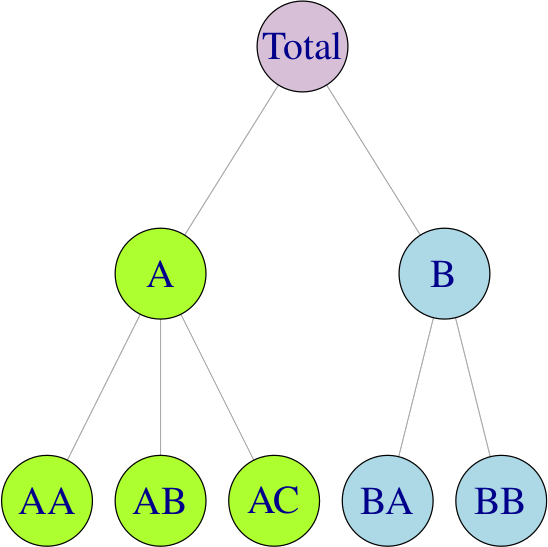
\includegraphics[height=5cm]{./assets/hts.png}
    \caption{An hierarchical set of time series. Picture taken from \cite{hyndman_forecasting_2021}.}
    \label{fig:hts}
  \end{figure}

\section{Hierarchical Forecast Reconciliation in Large-scale Settings}   \label{sec:ourwork}
Our main motivations of this paper are the limitations of prior work for problem settings with many time series.

\paragraph{Scaling issues with reconciliation methods}
In reconciliation methods, we see the following issues when scaling to many time series:
\begin{itemize}
  \item The reconciliation is performed as a \textit{post-processing} step, and thus has to be performed as an additional step after generating the base forecasts. Even though \(P\) in Eq.~\ref{eq:hfp} can be computed once using Eq.~\eqref{eq:p1}, the reconciliation still needs to be performed after each base forecast is produced. Also, \(P\) ideally is sparse \cite{bentaieb_regularized_2019}, but no reconciliation method guarantees this so computing Eq.~\ref{eq:hfp} will generally be a dense matrix-vector product that scales with the number of timeseries.
  \item For \textit{MinTShrink} \cite{wickramasuriya_optimal_2019}, estimating \(W\) according to the method of \cite{schafer_shrinkage_2005} is computationally expensive, as computing this estimate has a computational complexity of \(O(Nn^2)\), with \(N\) denoting the number of training samples used to compute the shrunk covariance estimate. In addition, the shrunk covariance estimate of \cite{schafer_shrinkage_2005} is not guaranteed to give consistent results in high-dimensional settings \cite{touloumis_nonparametric_2015}, making it less applicable for problem settings with many time series. Finally, the estimate for \(W\) will generally be a dense matrix, so we cannot make use of efficient sparse algorithms to solve Eq.~\eqref{eq:p1}. However, even for simpler, sparse choices of \(W\) (such as the identity matrix of \textit{OLS} \cite{hyndman_optimal_2011}), we still need to invert a matrix of size \(m^* \times m^*\) in order to solve Eq.~\eqref{eq:p1}, which becomes computationally costly for problems with many aggregations, which naturally arise in retail forecasting scenarios. For example, for the M5 retail forecasting competition \cite{makridakis_m5_2020}, \(m^*=12350\), even though there are only 3049 unique products in the dataset.  
  \item For \textit{ERM} and its regularized variants \cite{bentaieb_regularized_2019}, we need to either invert multiple dense matrices that scale quadratically with the number of time series, or we need to compute a Kronecker product that scales quadratically with the number of time series, followed by an expensive lasso search procedure. Improving the computational complexity of the \textit{ERM} methods is also mentioned in \cite{bentaieb_regularized_2019} as an avenue for future work.
\end{itemize}

\paragraph{Scaling issues with other methods}
\begin{itemize}
  \item SHARQ
  \item DeepVAR
\end{itemize}

\section{Sparse Gradients}
\begin{align}
  \textbf{y}_{t} &= S  \textbf{y}^n_{t} \nonumber \\
  \hat{\textbf{y}}_{t} &= S \hat{\textbf{y}}^n_{t} \nonumber \\
  L &= \frac{1}{m} \sum \left[ \frac{\frac{1}{2}(\textbf{y}_{t} - \hat{\textbf{y}}_{t})^2}{l \sum_{j=1}^n S_{ij}} \right]
\end{align}

\begin{align}
  \frac{\partial L}{\partial \hat{\textbf{y}}_{t}} &=  \left[ \frac{(\hat{\textbf{y}}_{t} - \textbf{y}_{t})}{l \sum_{j=1}^n S_{ij}} \right] \\
  \frac{\partial L}{\partial \hat{\textbf{y}}^n_{t}} &= \frac{\partial L}{d \hat{\textbf{y}}_{t}} S \\
  \frac{\partial^2 L}{\partial \hat{\textbf{y}}_{t}^{n, 2}} &= \mathbf{1}^n
\end{align}

\section{Experiments}
  \label{sec:experiments}
  In this section we empirically verify our theoretical results.\footnote{The code to reproduce our experiments can be found at LINK} First, we demonstrate how using our randomized aggregated loss improves forecasting performance by up to [x\%]. Then, we show that using our aggregated loss results in a reduction of bias and variance, as suggested by our theoretical result.

  \subsection{Public datasets}
    \label{subsec:publicdatasets}

  \subsection{Proprietary datasets}
    \label{subsec:proprietarydatasets}

\section{Discussion}
  \label{sec:discussion}


\section{Conclusion}
  \label{sec:conclusion}


\section*{Broader Impact}

  Positive: better forecasts

  Negative: implicitly our system may build on dependencies between time series that may be considered biased, or could potentially be discriminatory. 

\begin{ack}
  This research was (partially) funded by the Hybrid Intelligence Center, a 10-year program funded by the Dutch Ministry of Education, Culture and Science through the Netherlands Organisation for Scientific Research.\footnote{\url{https://www.hybrid-intelligence-centre.nl/}}

  All content represents the opinion of the authors, which is not necessarily shared or endorsed by their respective employers and/or sponsors.
  
  We thank the reviewers for their constructive feedback and help on improving our work. 

\end{ack}

\bibliographystyle{plainnat} 
\bibliography{lib}

\clearpage
\appendix

\end{document}
